\documentclass[1p]{elsarticle_modified}
%\bibliographystyle{elsarticle-num}

%\usepackage[colorlinks]{hyperref}
%\usepackage{abbrmath_seonhwa} %\Abb, \Ascr, \Acal ,\Abf, \Afrak
\usepackage{amsfonts}
\usepackage{amssymb}
\usepackage{amsmath}
\usepackage{amsthm}
\usepackage{scalefnt}
\usepackage{amsbsy}
\usepackage{kotex}
\usepackage{caption}
\usepackage{subfig}
\usepackage{color}
\usepackage{graphicx}
\usepackage{xcolor} %% white, black, red, green, blue, cyan, magenta, yellow
\usepackage{float}
\usepackage{setspace}
\usepackage{hyperref}

\usepackage{tikz}
\usetikzlibrary{arrows}

\usepackage{multirow}
\usepackage{array} % fixed length table
\usepackage{hhline}

%%%%%%%%%%%%%%%%%%%%%
\makeatletter
\renewcommand*\env@matrix[1][\arraystretch]{%
	\edef\arraystretch{#1}%
	\hskip -\arraycolsep
	\let\@ifnextchar\new@ifnextchar
	\array{*\c@MaxMatrixCols c}}
\makeatother %https://tex.stackexchange.com/questions/14071/how-can-i-increase-the-line-spacing-in-a-matrix
%%%%%%%%%%%%%%%

\usepackage[normalem]{ulem}

\newcommand{\msout}[1]{\ifmmode\text{\sout{\ensuremath{#1}}}\else\sout{#1}\fi}
%SOURCE: \msout is \stkout macro in https://tex.stackexchange.com/questions/20609/strikeout-in-math-mode

\newcommand{\cancel}[1]{
	\ifmmode
	{\color{red}\msout{#1}}
	\else
	{\color{red}\sout{#1}}
	\fi
}

\newcommand{\add}[1]{
	{\color{blue}\uwave{#1}}
}

\newcommand{\replace}[2]{
	\ifmmode
	{\color{red}\msout{#1}}{\color{blue}\uwave{#2}}
	\else
	{\color{red}\sout{#1}}{\color{blue}\uwave{#2}}
	\fi
}

\newcommand{\Sol}{\mathcal{S}} %segment
\newcommand{\D}{D} %diagram
\newcommand{\A}{\mathcal{A}} %arc


%%%%%%%%%%%%%%%%%%%%%%%%%%%%%5 test

\def\sl{\operatorname{\textup{SL}}(2,\Cbb)}
\def\psl{\operatorname{\textup{PSL}}(2,\Cbb)}
\def\quan{\mkern 1mu \triangleright \mkern 1mu}

\theoremstyle{definition}
\newtheorem{thm}{Theorem}[section]
\newtheorem{prop}[thm]{Proposition}
\newtheorem{lem}[thm]{Lemma}
\newtheorem{ques}[thm]{Question}
\newtheorem{cor}[thm]{Corollary}
\newtheorem{defn}[thm]{Definition}
\newtheorem{exam}[thm]{Example}
\newtheorem{rmk}[thm]{Remark}
\newtheorem{alg}[thm]{Algorithm}

\newcommand{\I}{\sqrt{-1}}
\begin{document}

%\begin{frontmatter}
%
%\title{Boundary parabolic representations of knots up to 8 crossings}
%
%%% Group authors per affiliation:
%\author{Yunhi Cho} 
%\address{Department of Mathematics, University of Seoul, Seoul, Korea}
%\ead{yhcho@uos.ac.kr}
%
%
%\author{Seonhwa Kim} %\fnref{s_kim}}
%\address{Center for Geometry and Physics, Institute for Basic Science, Pohang, 37673, Korea}
%\ead{ryeona17@ibs.re.kr}
%
%\author{Hyuk Kim}
%\address{Department of Mathematical Sciences, Seoul National University, Seoul 08826, Korea}
%\ead{hyukkim@snu.ac.kr}
%
%\author{Seokbeom Yoon}
%\address{Department of Mathematical Sciences, Seoul National University, Seoul, 08826,  Korea}
%\ead{sbyoon15@snu.ac.kr}
%
%\begin{abstract}
%We find all boundary parabolic representation of knots up to 8 crossings.
%
%\end{abstract}
%\begin{keyword}
%    \MSC[2010] 57M25 
%\end{keyword}
%
%\end{frontmatter}

%\linenumbers
%\tableofcontents
%
\newcommand\colored[1]{\textcolor{white}{\rule[-0.35ex]{0.8em}{1.4ex}}\kern-0.8em\color{red} #1}%
%\newcommand\colored[1]{\textcolor{white}{ #1}\kern-2.17ex	\textcolor{white}{ #1}\kern-1.81ex	\textcolor{white}{ #1}\kern-2.15ex\color{red}#1	}

{\Large $\underline{10_{158}~(K10n_{41})}$}

\setlength{\tabcolsep}{10pt}
\renewcommand{\arraystretch}{1.6}
\vspace{1cm}\begin{tabular}{m{100pt}>{\centering\arraybackslash}m{274pt}}
\multirow{5}{120pt}{
	\centering
	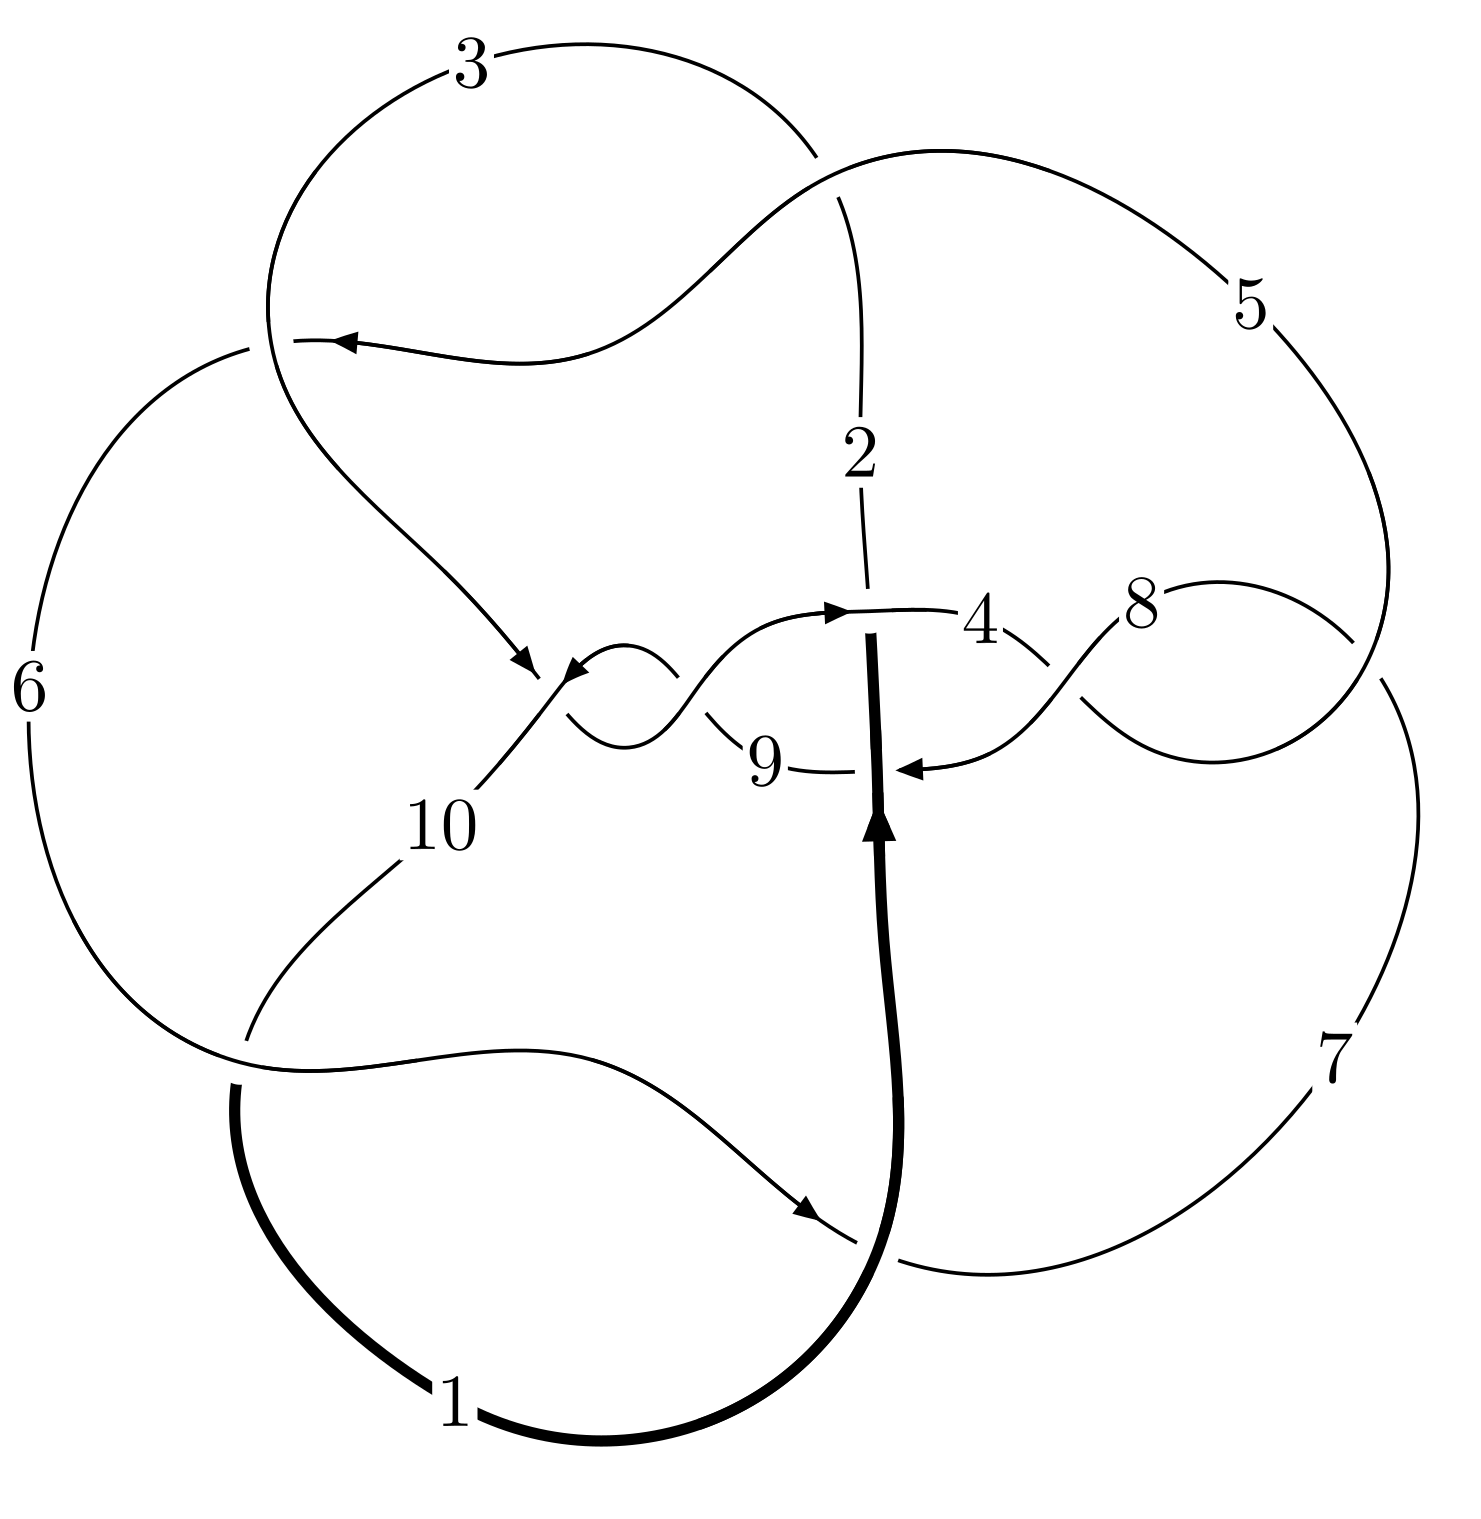
\includegraphics[width=112pt]{../../../GIT/diagram.site/Diagrams/png/242_10_158.png}\\
\ \ \ A knot diagram\footnotemark}&
\allowdisplaybreaks
\textbf{Linearized knot diagam} \\
\cline{2-2}
 &
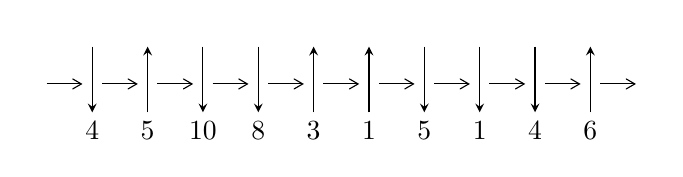
\begin{tikzpicture}[x=20pt, y=17pt]
	% nodes
	\node (C0) at (0, 0) {};
	\node (C1) at (1, 0) {};
	\node (C1U) at (1, +1) {};
	\node (C1D) at (1, -1) {4};

	\node (C2) at (2, 0) {};
	\node (C2U) at (2, +1) {};
	\node (C2D) at (2, -1) {5};

	\node (C3) at (3, 0) {};
	\node (C3U) at (3, +1) {};
	\node (C3D) at (3, -1) {10};

	\node (C4) at (4, 0) {};
	\node (C4U) at (4, +1) {};
	\node (C4D) at (4, -1) {8};

	\node (C5) at (5, 0) {};
	\node (C5U) at (5, +1) {};
	\node (C5D) at (5, -1) {3};

	\node (C6) at (6, 0) {};
	\node (C6U) at (6, +1) {};
	\node (C6D) at (6, -1) {1};

	\node (C7) at (7, 0) {};
	\node (C7U) at (7, +1) {};
	\node (C7D) at (7, -1) {5};

	\node (C8) at (8, 0) {};
	\node (C8U) at (8, +1) {};
	\node (C8D) at (8, -1) {1};

	\node (C9) at (9, 0) {};
	\node (C9U) at (9, +1) {};
	\node (C9D) at (9, -1) {4};

	\node (C10) at (10, 0) {};
	\node (C10U) at (10, +1) {};
	\node (C10D) at (10, -1) {6};
	\node (C11) at (11, 0) {};

	% arrows
	\draw[->,>={angle 60}]
	(C0) edge (C1) (C1) edge (C2) (C2) edge (C3) (C3) edge (C4) (C4) edge (C5) (C5) edge (C6) (C6) edge (C7) (C7) edge (C8) (C8) edge (C9) (C9) edge (C10) (C10) edge (C11) ;	\draw[->,>=stealth]
	(C1U) edge (C1D) (C2D) edge (C2U) (C3U) edge (C3D) (C4U) edge (C4D) (C5D) edge (C5U) (C6D) edge (C6U) (C7U) edge (C7D) (C8U) edge (C8D) (C9U) edge (C9D) (C10D) edge (C10U) ;
	\end{tikzpicture} \\
\hhline{~~} \\& 
\textbf{Solving Sequence} \\ \cline{2-2} 
 &
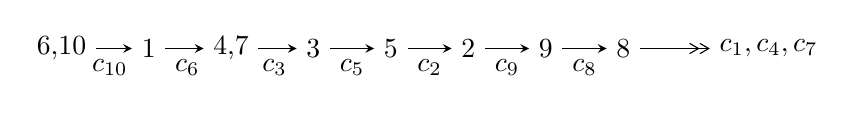
\begin{tikzpicture}[x=28pt, y=7pt]
	% node
	\node (A0) at (-1/8, 0) {6,10};
	\node (A1) at (1, 0) {1};
	\node (A2) at (33/16, 0) {4,7};
	\node (A3) at (25/8, 0) {3};
	\node (A4) at (33/8, 0) {5};
	\node (A5) at (41/8, 0) {2};
	\node (A6) at (49/8, 0) {9};
	\node (A7) at (57/8, 0) {8};
	\node (C1) at (1/2, -1) {$c_{10}$};
	\node (C2) at (3/2, -1) {$c_{6}$};
	\node (C3) at (21/8, -1) {$c_{3}$};
	\node (C4) at (29/8, -1) {$c_{5}$};
	\node (C5) at (37/8, -1) {$c_{2}$};
	\node (C6) at (45/8, -1) {$c_{9}$};
	\node (C7) at (53/8, -1) {$c_{8}$};
	\node (A8) at (9, 0) {$c_{1},c_{4},c_{7}$};

	% edge
	\draw[->,>=stealth]	
	(A0) edge (A1) (A1) edge (A2) (A2) edge (A3) (A3) edge (A4) (A4) edge (A5) (A5) edge (A6) (A6) edge (A7) ;
	\draw[->>,>={angle 60}]	
	(A7) edge (A8);
\end{tikzpicture} \\ 

\end{tabular} \\

\footnotetext{
The image of knot diagram is generated by the software ``\textbf{Draw programme}" developed by Andrew Bartholomew(\url{http://www.layer8.co.uk/maths/draw/index.htm\#Running-draw}), where we modified some parts for our purpose(\url{https://github.com/CATsTAILs/LinksPainter}).
}\phantom \\ \newline 
\centering \textbf{Ideals for irreducible components\footnotemark of $X_{\text{par}}$} 
 
\begin{align*}
I^u_{1}&=\langle 
17 u^{11}+20 u^{10}-54 u^9-54 u^8+116 u^7+92 u^6-101 u^5-48 u^4- u^3+16 u^2+37 b+5 u-10,\\
\phantom{I^u_{1}}&\phantom{= \langle  }-17 u^{11}-20 u^{10}+54 u^9+54 u^8-116 u^7-92 u^6+101 u^5+48 u^4+u^3-16 u^2+37 a-5 u-27,\\
\phantom{I^u_{1}}&\phantom{= \langle  }u^{12}+u^{11}-3 u^{10}-3 u^9+7 u^8+6 u^7-6 u^6-6 u^5+3 u^4+3 u^3+1\rangle \\
I^u_{2}&=\langle 
2201978 u^{15}-5194678 u^{14}+\cdots+19920857 b+76411393,\\
\phantom{I^u_{2}}&\phantom{= \langle  }-7295235 u^{15}+80490581 u^{14}+\cdots+378496283 a-1195533446,\;u^{16}- u^{15}+\cdots+2 u+19\rangle \\
I^u_{3}&=\langle 
- u^4+u^3+u^2+b- u,\;u^4- u^3- u^2+a+u+1,\;u^6- u^5-2 u^4+2 u^3+u^2- u+1\rangle \\
\\
\end{align*}
\raggedright * 3 irreducible components of $\dim_{\mathbb{C}}=0$, with total 34 representations.\\
\footnotetext{All coefficients of polynomials are rational numbers. But the coefficients are sometimes approximated in decimal forms when there is not enough margin.}
\newpage
\renewcommand{\arraystretch}{1}
\centering \section*{I. $I^u_{1}= \langle 17 u^{11}+20 u^{10}+\cdots+37 b-10,\;-17 u^{11}-20 u^{10}+\cdots+37 a-27,\;u^{12}+u^{11}+\cdots+3 u^3+1 \rangle$}
\flushleft \textbf{(i) Arc colorings}\\
\begin{tabular}{m{7pt} m{180pt} m{7pt} m{180pt} }
\flushright $a_{6}=$&$\begin{pmatrix}0\\u\end{pmatrix}$ \\
\flushright $a_{10}=$&$\begin{pmatrix}1\\0\end{pmatrix}$ \\
\flushright $a_{1}=$&$\begin{pmatrix}1\\- u^2\end{pmatrix}$ \\
\flushright $a_{4}=$&$\begin{pmatrix}0.459459 u^{11}+0.540541 u^{10}+\cdots+0.135135 u+0.729730\\-0.459459 u^{11}-0.540541 u^{10}+\cdots-0.135135 u+0.270270\end{pmatrix}$ \\
\flushright $a_{7}=$&$\begin{pmatrix}u\\- u^3+u\end{pmatrix}$ \\
\flushright $a_{3}=$&$\begin{pmatrix}1\\-0.459459 u^{11}-0.540541 u^{10}+\cdots-0.135135 u+0.270270\end{pmatrix}$ \\
\flushright $a_{5}=$&$\begin{pmatrix}- u\\0.0810811 u^{11}-0.0810811 u^{10}+\cdots+0.729730 u-0.459459\end{pmatrix}$ \\
\flushright $a_{2}=$&$\begin{pmatrix}- u^2+1\\-0.621622 u^{11}-0.378378 u^{10}+\cdots-0.594595 u+0.189189\end{pmatrix}$ \\
\flushright $a_{9}=$&$\begin{pmatrix}-0.945946 u^{11}-0.0540541 u^{10}+\cdots+0.486486 u+0.0270270\\1.40541 u^{11}+0.594595 u^{10}+\cdots-0.351351 u+0.702703\end{pmatrix}$ \\
\flushright $a_{8}=$&$\begin{pmatrix}-0.324324 u^{11}+0.324324 u^{10}+\cdots+1.08108 u-0.162162\\0.918919 u^{11}+0.0810811 u^{10}+\cdots+0.270270 u+0.459459\end{pmatrix}$\\&\end{tabular}
\flushleft \textbf{(ii) Obstruction class $= -1$}\\~\\
\flushleft \textbf{(iii) Cusp Shapes $= -\frac{50}{37} u^{11}-\frac{135}{37} u^{10}+\frac{87}{37} u^9+\frac{383}{37} u^8-\frac{191}{37} u^7-\frac{843}{37} u^6+\frac{25}{37} u^5+\frac{657}{37} u^4+\frac{127}{37} u^3-\frac{404}{37} u^2-\frac{117}{37} u-\frac{25}{37}$}\\~\\
\newpage\renewcommand{\arraystretch}{1}
\flushleft \textbf{(iv) u-Polynomials at the component}\newline \\
\begin{tabular}{m{50pt}|m{274pt}}
Crossings & \hspace{64pt}u-Polynomials at each crossing \\
\hline $$\begin{aligned}c_{1},c_{8}\end{aligned}$$&$\begin{aligned}
&u^{12}- u^{11}+\cdots-3 u+1
\end{aligned}$\\
\hline $$\begin{aligned}c_{2},c_{5},c_{6}\\c_{10}\end{aligned}$$&$\begin{aligned}
&u^{12}+u^{11}-3 u^{10}-3 u^9+7 u^8+6 u^7-6 u^6-6 u^5+3 u^4+3 u^3+1
\end{aligned}$\\
\hline $$\begin{aligned}c_{3},c_{9}\end{aligned}$$&$\begin{aligned}
&u^{12}+9 u^{11}+\cdots+96 u+16
\end{aligned}$\\
\hline $$\begin{aligned}c_{4},c_{7}\end{aligned}$$&$\begin{aligned}
&u^{12}-6 u^{11}+\cdots-10 u+4
\end{aligned}$\\
\hline
\end{tabular}\\~\\
\newpage\renewcommand{\arraystretch}{1}
\flushleft \textbf{(v) Riley Polynomials at the component}\newline \\
\begin{tabular}{m{50pt}|m{274pt}}
Crossings & \hspace{64pt}Riley Polynomials at each crossing \\
\hline $$\begin{aligned}c_{1},c_{8}\end{aligned}$$&$\begin{aligned}
&y^{12}-15 y^{11}+\cdots+7 y+1
\end{aligned}$\\
\hline $$\begin{aligned}c_{2},c_{5},c_{6}\\c_{10}\end{aligned}$$&$\begin{aligned}
&y^{12}-7 y^{11}+\cdots+6 y^2+1
\end{aligned}$\\
\hline $$\begin{aligned}c_{3},c_{9}\end{aligned}$$&$\begin{aligned}
&y^{12}+5 y^{11}+\cdots+896 y+256
\end{aligned}$\\
\hline $$\begin{aligned}c_{4},c_{7}\end{aligned}$$&$\begin{aligned}
&y^{12}+6 y^{11}+\cdots+20 y+16
\end{aligned}$\\
\hline
\end{tabular}\\~\\
\newpage\flushleft \textbf{(vi) Complex Volumes and Cusp Shapes}
$$\begin{array}{c|c|c}  
\text{Solutions to }I^u_{1}& \I (\text{vol} + \sqrt{-1}CS) & \text{Cusp shape}\\
 \hline 
\begin{aligned}
u &= -0.932110 + 0.403591 I \\
a &= \phantom{-}0.86095 - 1.68780 I \\
b &= \phantom{-}0.13905 + 1.68780 I\end{aligned}
 & \phantom{-}7.74885 - 1.69313 I & -0.90926 + 4.65688 I \\ \hline\begin{aligned}
u &= -0.932110 - 0.403591 I \\
a &= \phantom{-}0.86095 + 1.68780 I \\
b &= \phantom{-}0.13905 - 1.68780 I\end{aligned}
 & \phantom{-}7.74885 + 1.69313 I & -0.90926 - 4.65688 I \\ \hline\begin{aligned}
u &= \phantom{-}0.964469 + 0.359565 I \\
a &= -0.466137 - 0.540935 I \\
b &= \phantom{-}1.46614 + 0.54093 I\end{aligned}
 & -1.16607 + 4.31349 I & \phantom{-}1.88826 - 4.73148 I \\ \hline\begin{aligned}
u &= \phantom{-}0.964469 - 0.359565 I \\
a &= -0.466137 + 0.540935 I \\
b &= \phantom{-}1.46614 - 0.54093 I\end{aligned}
 & -1.16607 - 4.31349 I & \phantom{-}1.88826 + 4.73148 I \\ \hline\begin{aligned}
u &= -0.581296 + 0.573734 I \\
a &= -0.118591 + 0.442092 I \\
b &= \phantom{-}1.118590 - 0.442092 I\end{aligned}
 & -3.10204 + 1.08202 I & -2.61157 + 1.33940 I \\ \hline\begin{aligned}
u &= -0.581296 - 0.573734 I \\
a &= -0.118591 - 0.442092 I \\
b &= \phantom{-}1.118590 + 0.442092 I\end{aligned}
 & -3.10204 - 1.08202 I & -2.61157 - 1.33940 I \\ \hline\begin{aligned}
u &= \phantom{-}1.157820 + 0.740786 I \\
a &= \phantom{-}0.319275 + 1.332450 I \\
b &= \phantom{-}0.68073 - 1.33245 I\end{aligned}
 & -0.09105 + 5.46102 I & -0.77116 - 3.85424 I \\ \hline\begin{aligned}
u &= \phantom{-}1.157820 - 0.740786 I \\
a &= \phantom{-}0.319275 - 1.332450 I \\
b &= \phantom{-}0.68073 + 1.33245 I\end{aligned}
 & -0.09105 - 5.46102 I & -0.77116 + 3.85424 I \\ \hline\begin{aligned}
u &= \phantom{-}0.256008 + 0.492477 I \\
a &= \phantom{-}0.735049 + 0.459069 I \\
b &= \phantom{-}0.264951 - 0.459069 I\end{aligned}
 & -0.090701 + 1.098140 I & -1.42722 - 6.18957 I \\ \hline\begin{aligned}
u &= \phantom{-}0.256008 - 0.492477 I \\
a &= \phantom{-}0.735049 - 0.459069 I \\
b &= \phantom{-}0.264951 + 0.459069 I\end{aligned}
 & -0.090701 - 1.098140 I & -1.42722 + 6.18957 I\\
 \hline 
 \end{array}$$\newpage$$\begin{array}{c|c|c}  
\text{Solutions to }I^u_{1}& \I (\text{vol} + \sqrt{-1}CS) & \text{Cusp shape}\\
 \hline 
\begin{aligned}
u &= -1.36489 + 0.70235 I \\
a &= \phantom{-}0.169451 - 1.349320 I \\
b &= \phantom{-}0.83055 + 1.34932 I\end{aligned}
 & \phantom{-}1.63582 - 12.27120 I & \phantom{-}1.33095 + 7.21681 I \\ \hline\begin{aligned}
u &= -1.36489 - 0.70235 I \\
a &= \phantom{-}0.169451 + 1.349320 I \\
b &= \phantom{-}0.83055 - 1.34932 I\end{aligned}
 & \phantom{-}1.63582 + 12.27120 I & \phantom{-}1.33095 - 7.21681 I\\
 \hline 
 \end{array}$$\newpage\newpage\renewcommand{\arraystretch}{1}
\centering \section*{II. $I^u_{2}= \langle 2.20\times10^{6} u^{15}-5.19\times10^{6} u^{14}+\cdots+1.99\times10^{7} b+7.64\times10^{7},\;-7.30\times10^{6} u^{15}+8.05\times10^{7} u^{14}+\cdots+3.78\times10^{8} a-1.20\times10^{9},\;u^{16}- u^{15}+\cdots+2 u+19 \rangle$}
\flushleft \textbf{(i) Arc colorings}\\
\begin{tabular}{m{7pt} m{180pt} m{7pt} m{180pt} }
\flushright $a_{6}=$&$\begin{pmatrix}0\\u\end{pmatrix}$ \\
\flushright $a_{10}=$&$\begin{pmatrix}1\\0\end{pmatrix}$ \\
\flushright $a_{1}=$&$\begin{pmatrix}1\\- u^2\end{pmatrix}$ \\
\flushright $a_{4}=$&$\begin{pmatrix}0.0192743 u^{15}-0.212659 u^{14}+\cdots+0.532412 u+3.15864\\-0.110536 u^{15}+0.260766 u^{14}+\cdots+2.55924 u-3.83575\end{pmatrix}$ \\
\flushright $a_{7}=$&$\begin{pmatrix}u\\- u^3+u\end{pmatrix}$ \\
\flushright $a_{3}=$&$\begin{pmatrix}-0.0912621 u^{15}+0.0481069 u^{14}+\cdots+3.09165 u-0.677108\\-0.110536 u^{15}+0.260766 u^{14}+\cdots+2.55924 u-3.83575\end{pmatrix}$ \\
\flushright $a_{5}=$&$\begin{pmatrix}-0.0769980 u^{15}+0.306127 u^{14}+\cdots-1.09454 u+0.395782\\0.245201 u^{15}-0.534471 u^{14}+\cdots-4.85223 u+6.14044\end{pmatrix}$ \\
\flushright $a_{2}=$&$\begin{pmatrix}-0.489701 u^{15}+0.863952 u^{14}+\cdots+6.26646 u-3.26339\\0.294483 u^{15}-0.508467 u^{14}+\cdots-6.40955 u+4.64021\end{pmatrix}$ \\
\flushright $a_{9}=$&$\begin{pmatrix}-0.212645 u^{15}+0.307616 u^{14}+\cdots+2.68411 u-2.66285\\-0.110536 u^{15}+0.260766 u^{14}+\cdots+2.55924 u-2.83575\end{pmatrix}$ \\
\flushright $a_{8}=$&$\begin{pmatrix}-0.507128 u^{15}+0.816083 u^{14}+\cdots+9.09366 u-7.30305\\0.0690837 u^{15}-0.0661749 u^{14}+\cdots-2.60797 u+1.22994\end{pmatrix}$\\&\end{tabular}
\flushleft \textbf{(ii) Obstruction class $= -1$}\\~\\
\flushleft \textbf{(iii) Cusp Shapes $= -\frac{187108568}{378496283} u^{15}+\frac{381114024}{378496283} u^{14}+\cdots+\frac{1298769712}{378496283} u-\frac{136693666}{19920857}$}\\~\\
\newpage\renewcommand{\arraystretch}{1}
\flushleft \textbf{(iv) u-Polynomials at the component}\newline \\
\begin{tabular}{m{50pt}|m{274pt}}
Crossings & \hspace{64pt}u-Polynomials at each crossing \\
\hline $$\begin{aligned}c_{1},c_{8}\end{aligned}$$&$\begin{aligned}
&u^{16}-3 u^{15}+\cdots-10 u+1
\end{aligned}$\\
\hline $$\begin{aligned}c_{2},c_{5},c_{6}\\c_{10}\end{aligned}$$&$\begin{aligned}
&u^{16}- u^{15}+\cdots+2 u+19
\end{aligned}$\\
\hline $$\begin{aligned}c_{3},c_{9}\end{aligned}$$&$\begin{aligned}
&(u^2- u+1)^8
\end{aligned}$\\
\hline $$\begin{aligned}c_{4},c_{7}\end{aligned}$$&$\begin{aligned}
&(u^4+u^3+u^2+1)^4
\end{aligned}$\\
\hline
\end{tabular}\\~\\
\newpage\renewcommand{\arraystretch}{1}
\flushleft \textbf{(v) Riley Polynomials at the component}\newline \\
\begin{tabular}{m{50pt}|m{274pt}}
Crossings & \hspace{64pt}Riley Polynomials at each crossing \\
\hline $$\begin{aligned}c_{1},c_{8}\end{aligned}$$&$\begin{aligned}
&y^{16}-5 y^{15}+\cdots+88 y+1
\end{aligned}$\\
\hline $$\begin{aligned}c_{2},c_{5},c_{6}\\c_{10}\end{aligned}$$&$\begin{aligned}
&y^{16}-9 y^{15}+\cdots-1980 y+361
\end{aligned}$\\
\hline $$\begin{aligned}c_{3},c_{9}\end{aligned}$$&$\begin{aligned}
&(y^2+y+1)^8
\end{aligned}$\\
\hline $$\begin{aligned}c_{4},c_{7}\end{aligned}$$&$\begin{aligned}
&(y^4+y^3+3 y^2+2 y+1)^4
\end{aligned}$\\
\hline
\end{tabular}\\~\\
\newpage\flushleft \textbf{(vi) Complex Volumes and Cusp Shapes}
$$\begin{array}{c|c|c}  
\text{Solutions to }I^u_{2}& \I (\text{vol} + \sqrt{-1}CS) & \text{Cusp shape}\\
 \hline 
\begin{aligned}
u &= -0.921978 + 0.154671 I \\
a &= -1.18718 + 0.84702 I \\
b &= -0.500000 - 0.866025 I\end{aligned}
 & \phantom{-}5.14581 - 0.61478 I & \phantom{-}3.82674 - 1.44464 I \\ \hline\begin{aligned}
u &= -0.921978 - 0.154671 I \\
a &= -1.18718 - 0.84702 I \\
b &= -0.500000 + 0.866025 I\end{aligned}
 & \phantom{-}5.14581 + 0.61478 I & \phantom{-}3.82674 + 1.44464 I \\ \hline\begin{aligned}
u &= -1.000120 + 0.458209 I \\
a &= \phantom{-}0.23948 + 2.07179 I \\
b &= -0.500000 - 0.866025 I\end{aligned}
 & -1.85594 - 5.19385 I & \phantom{-}0.17326 + 6.02890 I \\ \hline\begin{aligned}
u &= -1.000120 - 0.458209 I \\
a &= \phantom{-}0.23948 - 2.07179 I \\
b &= -0.500000 + 0.866025 I\end{aligned}
 & -1.85594 + 5.19385 I & \phantom{-}0.17326 - 6.02890 I \\ \hline\begin{aligned}
u &= \phantom{-}0.740779 + 0.385723 I \\
a &= \phantom{-}0.60451 - 2.36642 I \\
b &= -0.500000 + 0.866025 I\end{aligned}
 & -1.85594 - 1.13408 I & \phantom{-}0.173262 - 0.899303 I \\ \hline\begin{aligned}
u &= \phantom{-}0.740779 - 0.385723 I \\
a &= \phantom{-}0.60451 + 2.36642 I \\
b &= -0.500000 - 0.866025 I\end{aligned}
 & -1.85594 + 1.13408 I & \phantom{-}0.173262 + 0.899303 I \\ \hline\begin{aligned}
u &= \phantom{-}0.656157 + 1.071140 I \\
a &= \phantom{-}0.546203 + 0.202750 I \\
b &= -0.500000 - 0.866025 I\end{aligned}
 & -1.85594 + 1.13408 I & \phantom{-}0.173262 + 0.899303 I \\ \hline\begin{aligned}
u &= \phantom{-}0.656157 - 1.071140 I \\
a &= \phantom{-}0.546203 - 0.202750 I \\
b &= -0.500000 + 0.866025 I\end{aligned}
 & -1.85594 - 1.13408 I & \phantom{-}0.173262 - 0.899303 I \\ \hline\begin{aligned}
u &= -0.291942 + 1.325280 I \\
a &= \phantom{-}0.328801 - 0.073667 I \\
b &= -0.500000 + 0.866025 I\end{aligned}
 & -1.85594 + 5.19385 I & \phantom{-}0.17326 - 6.02890 I \\ \hline\begin{aligned}
u &= -0.291942 - 1.325280 I \\
a &= \phantom{-}0.328801 + 0.073667 I \\
b &= -0.500000 - 0.866025 I\end{aligned}
 & -1.85594 - 5.19385 I & \phantom{-}0.17326 + 6.02890 I\\
 \hline 
 \end{array}$$\newpage$$\begin{array}{c|c|c}  
\text{Solutions to }I^u_{2}& \I (\text{vol} + \sqrt{-1}CS) & \text{Cusp shape}\\
 \hline 
\begin{aligned}
u &= \phantom{-}1.126160 + 0.776883 I \\
a &= -0.398018 - 0.407492 I \\
b &= -0.500000 + 0.866025 I\end{aligned}
 & \phantom{-}5.14581 + 3.44499 I & \phantom{-}3.82674 - 8.37284 I \\ \hline\begin{aligned}
u &= \phantom{-}1.126160 - 0.776883 I \\
a &= -0.398018 + 0.407492 I \\
b &= -0.500000 - 0.866025 I\end{aligned}
 & \phantom{-}5.14581 - 3.44499 I & \phantom{-}3.82674 + 8.37284 I \\ \hline\begin{aligned}
u &= -1.367540 + 0.181274 I \\
a &= -0.383277 + 1.317030 I \\
b &= -0.500000 - 0.866025 I\end{aligned}
 & \phantom{-}5.14581 - 3.44499 I & \phantom{-}3.82674 + 8.37284 I \\ \hline\begin{aligned}
u &= -1.367540 - 0.181274 I \\
a &= -0.383277 - 1.317030 I \\
b &= -0.500000 + 0.866025 I\end{aligned}
 & \phantom{-}5.14581 + 3.44499 I & \phantom{-}3.82674 - 8.37284 I \\ \hline\begin{aligned}
u &= \phantom{-}1.55848 + 0.24344 I \\
a &= -0.092631 - 0.872701 I \\
b &= -0.500000 + 0.866025 I\end{aligned}
 & \phantom{-}5.14581 + 0.61478 I & \phantom{-}3.82674 + 1.44464 I \\ \hline\begin{aligned}
u &= \phantom{-}1.55848 - 0.24344 I \\
a &= -0.092631 + 0.872701 I \\
b &= -0.500000 - 0.866025 I\end{aligned}
 & \phantom{-}5.14581 - 0.61478 I & \phantom{-}3.82674 - 1.44464 I\\
 \hline 
 \end{array}$$\newpage\newpage\renewcommand{\arraystretch}{1}
\centering \section*{III. $I^u_{3}= \langle - u^4+u^3+u^2+b- u,\;u^4- u^3- u^2+a+u+1,\;u^6- u^5-2 u^4+2 u^3+u^2- u+1 \rangle$}
\flushleft \textbf{(i) Arc colorings}\\
\begin{tabular}{m{7pt} m{180pt} m{7pt} m{180pt} }
\flushright $a_{6}=$&$\begin{pmatrix}0\\u\end{pmatrix}$ \\
\flushright $a_{10}=$&$\begin{pmatrix}1\\0\end{pmatrix}$ \\
\flushright $a_{1}=$&$\begin{pmatrix}1\\- u^2\end{pmatrix}$ \\
\flushright $a_{4}=$&$\begin{pmatrix}- u^4+u^3+u^2- u-1\\u^4- u^3- u^2+u\end{pmatrix}$ \\
\flushright $a_{7}=$&$\begin{pmatrix}u\\- u^3+u\end{pmatrix}$ \\
\flushright $a_{3}=$&$\begin{pmatrix}-1\\u^4- u^3- u^2+u\end{pmatrix}$ \\
\flushright $a_{5}=$&$\begin{pmatrix}- u\\u^5- u^4- u^3+u^2+u\end{pmatrix}$ \\
\flushright $a_{2}=$&$\begin{pmatrix}u^2-1\\- u^2+1\end{pmatrix}$ \\
\flushright $a_{9}=$&$\begin{pmatrix}u^4- u^3-2 u^2+2 u+1\\u^2- u\end{pmatrix}$ \\
\flushright $a_{8}=$&$\begin{pmatrix}u^4- u^3- u^2+2 u\\- u^4+2 u^2- u\end{pmatrix}$\\&\end{tabular}
\flushleft \textbf{(ii) Obstruction class $= 1$}\\~\\
\flushleft \textbf{(iii) Cusp Shapes $= -2 u^5- u^4+6 u^3+3 u^2-7 u+3$}\\~\\
\newpage\renewcommand{\arraystretch}{1}
\flushleft \textbf{(iv) u-Polynomials at the component}\newline \\
\begin{tabular}{m{50pt}|m{274pt}}
Crossings & \hspace{64pt}u-Polynomials at each crossing \\
\hline $$\begin{aligned}c_{1},c_{8}\end{aligned}$$&$\begin{aligned}
&u^6- u^5-2 u^3+2 u^2+1
\end{aligned}$\\
\hline $$\begin{aligned}c_{2},c_{6}\end{aligned}$$&$\begin{aligned}
&u^6+u^5-2 u^4-2 u^3+u^2+u+1
\end{aligned}$\\
\hline $$\begin{aligned}c_{3}\end{aligned}$$&$\begin{aligned}
&u^6+2 u^4+2 u^3+u+1
\end{aligned}$\\
\hline $$\begin{aligned}c_{4}\end{aligned}$$&$\begin{aligned}
&u^6- u^5+3 u^4-2 u^3+3 u^2+1
\end{aligned}$\\
\hline $$\begin{aligned}c_{5},c_{10}\end{aligned}$$&$\begin{aligned}
&u^6- u^5-2 u^4+2 u^3+u^2- u+1
\end{aligned}$\\
\hline $$\begin{aligned}c_{7}\end{aligned}$$&$\begin{aligned}
&u^6+u^5+3 u^4+2 u^3+3 u^2+1
\end{aligned}$\\
\hline $$\begin{aligned}c_{9}\end{aligned}$$&$\begin{aligned}
&u^6+2 u^4-2 u^3- u+1
\end{aligned}$\\
\hline
\end{tabular}\\~\\
\newpage\renewcommand{\arraystretch}{1}
\flushleft \textbf{(v) Riley Polynomials at the component}\newline \\
\begin{tabular}{m{50pt}|m{274pt}}
Crossings & \hspace{64pt}Riley Polynomials at each crossing \\
\hline $$\begin{aligned}c_{1},c_{8}\end{aligned}$$&$\begin{aligned}
&y^6- y^5-2 y^3+4 y^2+4 y+1
\end{aligned}$\\
\hline $$\begin{aligned}c_{2},c_{5},c_{6}\\c_{10}\end{aligned}$$&$\begin{aligned}
&y^6-5 y^5+10 y^4-8 y^3+y^2+y+1
\end{aligned}$\\
\hline $$\begin{aligned}c_{3},c_{9}\end{aligned}$$&$\begin{aligned}
&y^6+4 y^5+4 y^4-2 y^3- y+1
\end{aligned}$\\
\hline $$\begin{aligned}c_{4},c_{7}\end{aligned}$$&$\begin{aligned}
&y^6+5 y^5+11 y^4+16 y^3+15 y^2+6 y+1
\end{aligned}$\\
\hline
\end{tabular}\\~\\
\newpage\flushleft \textbf{(vi) Complex Volumes and Cusp Shapes}
$$\begin{array}{c|c|c}  
\text{Solutions to }I^u_{3}& \I (\text{vol} + \sqrt{-1}CS) & \text{Cusp shape}\\
 \hline 
\begin{aligned}
u &= -1.099190 + 0.287563 I \\
a &= -0.69782 + 1.52185 I \\
b &= -0.30218 - 1.52185 I\end{aligned}
 & \phantom{-}8.54916 - 1.24964 I & \phantom{-}7.95941 - 0.00232 I \\ \hline\begin{aligned}
u &= -1.099190 - 0.287563 I \\
a &= -0.69782 - 1.52185 I \\
b &= -0.30218 + 1.52185 I\end{aligned}
 & \phantom{-}8.54916 + 1.24964 I & \phantom{-}7.95941 + 0.00232 I \\ \hline\begin{aligned}
u &= \phantom{-}0.264925 + 0.576623 I \\
a &= -1.74836 - 0.18113 I \\
b &= \phantom{-}0.748359 + 0.181129 I\end{aligned}
 & -2.37427 + 2.84527 I & -1.26269 - 3.26816 I \\ \hline\begin{aligned}
u &= \phantom{-}0.264925 - 0.576623 I \\
a &= -1.74836 + 0.18113 I \\
b &= \phantom{-}0.748359 - 0.181129 I\end{aligned}
 & -2.37427 - 2.84527 I & -1.26269 + 3.26816 I \\ \hline\begin{aligned}
u &= \phantom{-}1.334260 + 0.378781 I \\
a &= -0.553818 - 0.708238 I \\
b &= -0.446182 + 0.708238 I\end{aligned}
 & \phantom{-}5.33965 + 2.32699 I & \phantom{-}5.80328 - 1.20156 I \\ \hline\begin{aligned}
u &= \phantom{-}1.334260 - 0.378781 I \\
a &= -0.553818 + 0.708238 I \\
b &= -0.446182 - 0.708238 I\end{aligned}
 & \phantom{-}5.33965 - 2.32699 I & \phantom{-}5.80328 + 1.20156 I\\
 \hline 
 \end{array}$$\newpage
\newpage\renewcommand{\arraystretch}{1}
\centering \section*{ IV. u-Polynomials}
\begin{tabular}{m{50pt}|m{274pt}}
Crossings & \hspace{64pt}u-Polynomials at each crossing \\
\hline $$\begin{aligned}c_{1},c_{8}\end{aligned}$$&$\begin{aligned}
&(u^6- u^5-2 u^3+2 u^2+1)(u^{12}- u^{11}+\cdots-3 u+1)\\
&\cdot(u^{16}-3 u^{15}+\cdots-10 u+1)
\end{aligned}$\\
\hline $$\begin{aligned}c_{2},c_{6}\end{aligned}$$&$\begin{aligned}
&(u^6+u^5-2 u^4-2 u^3+u^2+u+1)\\
&\cdot(u^{12}+u^{11}-3 u^{10}-3 u^9+7 u^8+6 u^7-6 u^6-6 u^5+3 u^4+3 u^3+1)\\
&\cdot(u^{16}- u^{15}+\cdots+2 u+19)
\end{aligned}$\\
\hline $$\begin{aligned}c_{3}\end{aligned}$$&$\begin{aligned}
&((u^2- u+1)^8)(u^6+2 u^4+2 u^3+u+1)(u^{12}+9 u^{11}+\cdots+96 u+16)
\end{aligned}$\\
\hline $$\begin{aligned}c_{4}\end{aligned}$$&$\begin{aligned}
&(u^4+u^3+u^2+1)^4(u^6- u^5+3 u^4-2 u^3+3 u^2+1)\\
&\cdot(u^{12}-6 u^{11}+\cdots-10 u+4)
\end{aligned}$\\
\hline $$\begin{aligned}c_{5},c_{10}\end{aligned}$$&$\begin{aligned}
&(u^6- u^5-2 u^4+2 u^3+u^2- u+1)\\
&\cdot(u^{12}+u^{11}-3 u^{10}-3 u^9+7 u^8+6 u^7-6 u^6-6 u^5+3 u^4+3 u^3+1)\\
&\cdot(u^{16}- u^{15}+\cdots+2 u+19)
\end{aligned}$\\
\hline $$\begin{aligned}c_{7}\end{aligned}$$&$\begin{aligned}
&(u^4+u^3+u^2+1)^4(u^6+u^5+3 u^4+2 u^3+3 u^2+1)\\
&\cdot(u^{12}-6 u^{11}+\cdots-10 u+4)
\end{aligned}$\\
\hline $$\begin{aligned}c_{9}\end{aligned}$$&$\begin{aligned}
&((u^2- u+1)^8)(u^6+2 u^4-2 u^3- u+1)(u^{12}+9 u^{11}+\cdots+96 u+16)
\end{aligned}$\\
\hline
\end{tabular}\newpage\renewcommand{\arraystretch}{1}
\centering \section*{ V. Riley Polynomials}
\begin{tabular}{m{50pt}|m{274pt}}
Crossings & \hspace{64pt}Riley Polynomials at each crossing \\
\hline $$\begin{aligned}c_{1},c_{8}\end{aligned}$$&$\begin{aligned}
&(y^6- y^5-2 y^3+4 y^2+4 y+1)(y^{12}-15 y^{11}+\cdots+7 y+1)\\
&\cdot(y^{16}-5 y^{15}+\cdots+88 y+1)
\end{aligned}$\\
\hline $$\begin{aligned}c_{2},c_{5},c_{6}\\c_{10}\end{aligned}$$&$\begin{aligned}
&(y^6-5 y^5+10 y^4-8 y^3+y^2+y+1)(y^{12}-7 y^{11}+\cdots+6 y^2+1)\\
&\cdot(y^{16}-9 y^{15}+\cdots-1980 y+361)
\end{aligned}$\\
\hline $$\begin{aligned}c_{3},c_{9}\end{aligned}$$&$\begin{aligned}
&(y^2+y+1)^8(y^6+4 y^5+4 y^4-2 y^3- y+1)\\
&\cdot(y^{12}+5 y^{11}+\cdots+896 y+256)
\end{aligned}$\\
\hline $$\begin{aligned}c_{4},c_{7}\end{aligned}$$&$\begin{aligned}
&(y^4+y^3+3 y^2+2 y+1)^4(y^6+5 y^5+11 y^4+16 y^3+15 y^2+6 y+1)\\
&\cdot(y^{12}+6 y^{11}+\cdots+20 y+16)
\end{aligned}$\\
\hline
\end{tabular}
\vskip 2pc
\end{document}